\chapter{Memory}

\label{ch:memory}

Everything else in this manual is about work: runs, rows, graphs, gates. This chapter is about
what survives the work — what pii remembers after a run ends, how it is found again, why some of
it fades, and what an operator should check when memory looks wrong. Scattered in earlier
chapters you will have seen memory mentioned next to the stores; that was a reference. This is the
chapter.

The short version, before the detail: \textbf{pii does not remember conversations. It remembers
documents.} A document is a piece of text with a layer, a kind, a set of concepts, and an id
derived from its own content. Nothing is remembered by being said; something is remembered by
being written, and writing the same text twice is the same document.

\section{The four things a document carries}

\begin{center}
\resizebox{\linewidth}{!}{
\begin{tikzpicture}[node distance=9mm and 13mm]
  \node[b] (id) {id\\\scriptsize blake3(text)[..16]};
  \node[b, right=of id] (layer) {layer\\\scriptsize L1 · L2 · L3};
  \node[b, right=of layer] (kind) {kind\\\scriptsize atom · scene · persona · skill};
  \node[b, below=of layer] (concepts) {concepts\\\scriptsize the words the graph lane can reach};
  \node[s, below=of id] (store) {mem store\\\scriptsize documents · edges};
  \node[p, right=of concepts] (note) {a doc without concepts is invisible to one of the three lanes};
  \draw[f] (id) -- (store);
  \draw[f] (layer) -- (store);
  \draw[sf] (concepts) -- (store);
  \draw[bk] (note) -- (concepts);
\end{tikzpicture}}
\captionof{figure}{The four fields that matter operationally. The id is derived, not assigned: two puts of the same text produce one document.}
\end{center}

Because the id is the hash of the text, \texttt{pii memory put} is \emph{idempotent}: writing the
same sentence twice does not create two memories, it rewrites one. That is also why editing a
memory means writing a new document — the text changed, so the id changed — and why a correction
appears as a new document rather than a modification of the old one.

\section{The three layers, and what each is for}

\begin{center}
\resizebox{\linewidth}{!}{
\begin{tikzpicture}[node distance=10mm and 8mm]
  \node[b, fill=orange!10, minimum width=3.4cm] (l1) {L1 — atoms\\\scriptsize one fact with its evidence};
  \node[b, fill=blue!8, below=of l1, minimum width=3.4cm] (l2) {L2 — scenes\\\scriptsize distilled summaries of related atoms};
  \node[b, fill=purple!10, below=of l2, minimum width=3.4cm] (l3) {L3 — skills and persona\\\scriptsize what pii does, and who it is for};
  \draw[f] (l1) -- node[p,right]{consolidation} (l2);
  \draw[f] (l2) -- node[p,right]{consolidation} (l3);
  \draw[sf] (l1.east) to[bend left=28] node[p,right]{never skips a layer} (l3.east);
\end{tikzpicture}}
\captionof{figure}{Consolidation moves upward and never backward. An atom is not a scene that lost detail; a scene is a set of atoms that agreed.}
\end{center}

The layers are not storage tiers — they are kinds of claim. An \textbf{atom} is one fact with
evidence: a single observation it would be wrong to generalise from. A \textbf{scene} is a
distillation of several atoms that share concepts: it says what the atoms together mean. \textbf{L3}
holds skills --- procedures pii can follow --- and the persona document, which is the one kind that
never decays.

Two consequences an operator should hold on to. First, a scene is derived: if you delete every
atom behind it, the scene remains but its evidence is gone, which is a reason to archive rather
than delete. Second, \texttt{same\_layer\_only} is on: consolidation will not merge an atom into
a scene, so a half-finished idea stays an atom until it earns its way up.

\section{How a memory is found: three lanes, one ranked list}

A search does not consult one index. Three independent lanes each produce candidates, and their
rankings are fused.

\begin{center}
\resizebox{\linewidth}{!}{
\begin{tikzpicture}[node distance=8mm and 11mm]
  \node[b] (q) {query};
  \node[b, below=of q, xshift=-4.6cm] (bm) {BM25 lane\\\scriptsize token overlap};
  \node[b, below=of q] (vec) {vector lane\\\scriptsize embeddings, int8};
  \node[b, below=of q, xshift=4.6cm] (gr) {graph lane\\\scriptsize concepts → neighbours};
  \node[b, below=of vec] (rrf) {RRF fusion\\\scriptsize k = 60};
  \node[v, below=of rrf] (decay) {decay?};
  \node[b, below=of decay] (ranked) {ranked hits\\\scriptsize with the lanes that ran};
  \draw[f] (q) -- (bm); \draw[f] (q) -- (vec); \draw[f] (q) -- (gr);
  \draw[f] (bm) -- (rrf); \draw[f] (vec) -- (rrf); \draw[f] (gr) -- (rrf);
  \draw[f] (rrf) -- (decay); \draw[f] (decay) -- (ranked);
\end{tikzpicture}}
\captionof{figure}{Fusion by rank, not by score. Reciprocal-rank fusion is used because the three lanes produce scores on incomparable scales — BM25 counts terms, cosine sits in $[-1,1]$, the graph lane counts hops.}
\end{center}

\textbf{Reciprocal-rank fusion} with $k = 60$ combines them: each lane contributes
$1/(k + \text{rank})$ per hit, and the sums decide the order. The practical effect is that a
document ranked first by one lane beats a document ranked fifth by all three, which is the
behaviour you want when one lane is much more confident than the rest.

Then decay is applied per kind, and here is the first thing that surprises operators:

\begin{center}
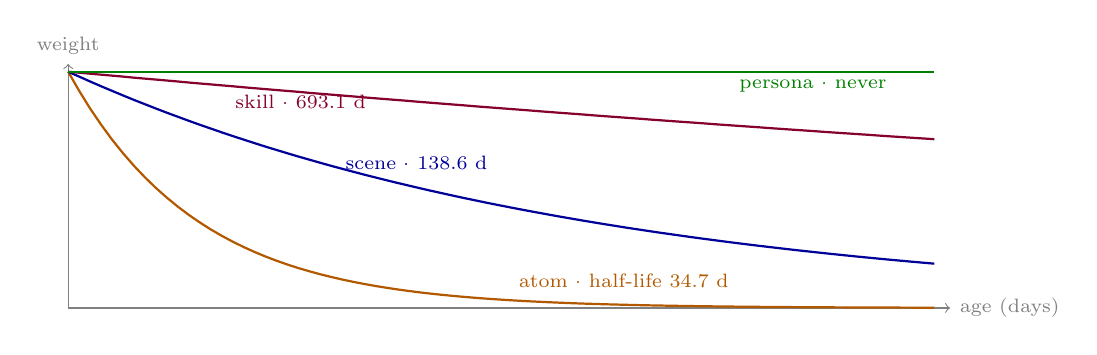
\begin{tikzpicture}[x=1cm, y=1cm]
  \draw[->, gray] (0,0) -- (11.2,0) node[right, font=\scriptsize] {age (days)};
  \draw[->, gray] (0,0) -- (0,3.1) node[above, font=\scriptsize] {weight};
  \draw[thick, orange!70!black] plot[domain=0:11, samples=80] (\x, {3*exp(-0.02*\x*30.4)});
  \draw[thick, blue!60!black]  plot[domain=0:11, samples=80] (\x, {3*exp(-0.005*\x*30.4)});
  \draw[thick, purple!70!black] plot[domain=0:11, samples=80] (\x, {3*exp(-0.001*\x*30.4)});
  \draw[thick, green!50!black] (0,3) -- (11,3);
  \node[font=\scriptsize, orange!70!black, right] at (5.6,0.35) {atom · half-life 34.7 d};
  \node[font=\scriptsize, blue!60!black, right] at (3.4,1.85) {scene · 138.6 d};
  \node[font=\scriptsize, purple!70!black, right] at (2.0,2.62) {skill · 693.1 d};
  \node[font=\scriptsize, green!50!black, right] at (8.4,2.82) {persona · never};
\end{tikzpicture}
\captionof{figure}{Decay is exponential, $\mathrm{score}\times e^{-\lambda\,\text{age}}$, with $\lambda$ fixed per kind. The half-lives are computed from the constants in the crate: 0.693/0.02, 0.693/0.005, 0.693/0.001.}
\end{center}

An atom written a month ago carries roughly half the weight of one written today; a skill written
two years ago still carries most of its weight. Decay reorders results, it does not delete
anything --- deletion is retention's job, and it is a separate mechanism (chapter~4).

\section{The graph lane, and why it often contributes nothing}

This is the intricacy most worth knowing, because it produces the most confusing symptom: a search
that returns obviously-related documents from BM25 and from vectors, while the graph lane appears
in the response and adds nothing.

The graph lane fires only when \emph{a query token is already a concept head present in the edge
table} --- that is, when some earlier document was written with that word in its concept list.
Free-text queries against documents stored without explicit concepts produce no query concepts at
all, so the lane contributes nothing.

\begin{center}
\resizebox{\linewidth}{!}{
\begin{tikzpicture}[node distance=8mm and 12mm]
  \node[b] (query) {query token\\\scriptsize "retention"};
  \node[v, right=of query] (isconcept) {a concept head?};
  \node[b, right=of isconcept, yshift=9mm] (expand) {expand to neighbours};
  \node[b, right=of isconcept, yshift=-9mm] (nothing) {lane contributes nothing};
  \node[b, right=of expand] (hits) {hits, ranked by hops};
  \draw[f] (query) -- (isconcept);
  \draw[f] (isconcept) -- node[p,above]{yes} (expand);
  \draw[f] (isconcept) -- node[p,below]{no} (nothing);
  \draw[f] (expand) -- (hits);
\end{tikzpicture}}
\captionof{figure}{The lane reports that it RAN either way. ``Ran'' is not ``hit'' — the response lists the lanes that were consulted, not the lanes that found something.}
\end{center}

The operational reading: if the graph lane never contributes on your store, your documents were
written without concepts. \texttt{pii memory put} takes the text; the concept list is what makes a
document reachable by association. Writing facts through the fact path records concepts, and that
is how a store becomes navigable rather than merely searchable.

\section{Consolidation: when many atoms become one scene}

Consolidation is the process that turns atoms into a scene. It is deliberately conservative, and
each of its limits is worth knowing because each one explains a scene that never appeared.

\begin{longtable}{@{}p{0.34\textwidth}p{0.20\textwidth}p{0.36\textwidth}@{}}
  \toprule
  \textbf{Rule} & \textbf{Value} & \textbf{What it means to an operator} \\
  \midrule
  \endhead
  shared concepts & at least 2 & a single shared word is never enough to merge \\
  concept Jaccard & at least 0.15 & the two documents must be about mostly the same thing \\
  negation window & 8 tokens & a ``not'' near a shared concept vetoes the merge \\
  candidate cap & 200 & generation stops at 200 and says so in the report \\
  same layer only & on & an atom is never merged into a scene \\
  archive after & configured days & documents past their last use are archived, not deleted \\
  \bottomrule
\end{longtable}

The negation window is the one that saves you: ``the disk floor is 12\,GB'' and ``the disk floor is
not 12\,GB'' share every concept, and would otherwise consolidate into a scene that asserts both.

\section{The commands, and what each one touches}

\begin{longtable}{@{}p{0.26\textwidth}p{0.40\textwidth}p{0.26\textwidth}@{}}
  \toprule
  \textbf{Command} & \textbf{What it does} & \textbf{Reads / writes} \\
  \midrule
  \endhead
  \texttt{memory search} & fused search over the three lanes, returns hits and the lanes that ran & reads documents and edges \\
  \texttt{memory put} & writes a document; the id is the content hash, so a repeat is a no-op & writes one document \\
  \texttt{memory learn} & records an outcome as a document & writes one document \\
  \texttt{memory tiers} & what sits in L1, L2 and L3 & reads only \\
  \texttt{memory entity} & creates or reads an entity in the entity graph & writes entities \\
  \texttt{memory link} & creates an edge between entities & writes edges \\
  \texttt{memory neighbours} & the entities adjacent to one entity & reads edges \\
  \texttt{memory consolidate} & generates candidate merges under the rules above & writes scenes, archives \\
  \texttt{memory compact} & removes superseded versions of a document & writes \\
  \texttt{memory show} & one document, in full, with its metadata & reads \\
  \texttt{memory archive} / \texttt{restore} & takes a document out of search, or puts it back & writes \\
  \bottomrule
\end{longtable}

Most of these go through the daemon, because the daemon is the only writer. If you are told
\texttt{uds.connect.failed}, the daemon is down --- that is a supervision problem (chapter~2), not
a memory problem, and it is worth saying plainly because the error names a socket rather than the
cause.

\section{What goes wrong, in the order you will meet it}

\begin{longtable}{@{}p{0.30\textwidth}p{0.34\textwidth}p{0.28\textwidth}@{}}
  \toprule
  \textbf{Symptom} & \textbf{Cause} & \textbf{What to do} \\
  \midrule
  \endhead
  results are stale but present & decay, not deletion & search again with a recency bias, or re-put the fact \\
  a fact is gone & retention swept it, or it was archived & \texttt{memory show} the id; restore from backup if needed \\
  the graph lane never contributes & documents were written without concepts & write facts through the fact path \\
  the vector lane is skipped & no embedder configured, or zero dimensions & the response marks itself degraded; BM25 and the graph still answer \\
  two documents say the same thing & the text differed by a character & the ids differ by design; consolidate or archive \\
  a scene asserts something odd & merged atoms that disagreed & the negation window covers only 8 tokens; tighten the concepts \\
  search is slow & a large store with no compact & run \texttt{memory compact}, then measure again \\
  \bottomrule
\end{longtable}

\section{How memory is bounded}

Memory is bounded in four independent ways, and an administrator should know which one is doing
the work on their host:

\begin{center}
\resizebox{\linewidth}{!}{
\begin{tikzpicture}[node distance=8mm and 10mm]
  \node[b] (write) {writes\\\scriptsize put · learn · consolidate};
  \node[b, right=of write] (docs) {documents\\\scriptsize content-addressed};
  \node[v, right=of docs] (bound) {bounded by?};
  \node[b, above=of bound, yshift=2mm] (ret) {retention\\\scriptsize age-based sweep};
  \node[b, right=of bound, yshift=9mm] (comp) {compaction\\\scriptsize superseded versions};
  \node[b, right=of bound, yshift=-3mm] (arch) {archival\\\scriptsize last-use age};
  \node[b, below=of bound] (disk) {the disk floor\\\scriptsize refuses before it is full};
  \draw[f] (write) -- (docs); \draw[f] (docs) -- (bound);
  \draw[sf] (bound) -- (ret); \draw[sf] (bound) -- (comp);
  \draw[sf] (bound) -- (arch); \draw[sf] (bound) -- (disk);
\end{tikzpicture}}
\captionof{figure}{Four bounds, four mechanisms, four different failure modes. ``Memory is full'' is never one thing; the question is which bound fired.}
\end{center}

The order to investigate: \texttt{pii store df} first (how big it actually is), then retention
(chapter~4) for what age has swept, then compaction for how much is superseded copies, then
archival for what consolidation moved aside. Only then is it a capacity question rather than a
policy one.
